\documentclass[11pt,a4paper]{article}
\usepackage[utf8]{inputenc}
\usepackage[T1]{fontenc}
\usepackage{lmodern}
\usepackage[margin=2.2cm]{geometry}
\usepackage{amsmath,amssymb}
\usepackage{graphicx}
\usepackage{booktabs}
\usepackage{siunitx}
\usepackage{caption}
\usepackage{float}
\usepackage{xcolor}
\usepackage{listings}
\usepackage[hidelinks]{hyperref}

\graphicspath{{../tutorial/plots/}{../project/plots/}}
\setlength{\emergencystretch}{2em}
\sisetup{detect-all, group-separator={\,}, group-minimum-digits=5}
\captionsetup{font=small,labelfont=bf}
\makeatletter\newcommand{\rowsinput}[1]{\@@input #1 }\makeatother
\lstset{basicstyle=\ttfamily\footnotesize, columns=fixed, keepspaces=true, frame=single, breaklines=true}

\title{\textbf{Assignment 3 -- Stability lobes and slot milling}\\[4pt]
\large Multi-Agent System for Smart Machining (ECIU micro-module, INSA Toulouse)}
\author{Daniele Trisotto}
\date{\today}

\begin{document}
\maketitle

\begin{abstract}
This report studies regenerative chatter in milling with stability lobes, first on a
tutorial case and then on a slot milling project.
In the tutorial (finish milling of a thin 6061-T6 wall), the analytical model of
Altintas \& Budak gives an unconditional limit of \SI{4.53}{mm}. The numerical
semi-discretization method confirms the Hopf lobes but shows a flip lobe, caused by the
interrupted cut, at a tooth pass frequency equal to twice the natural frequency, with a
limit of only \SI{2.4}{mm}; with a helix angle of \SI{45}{\degree} it becomes an island
repeated every axial pitch.
In the project, a $\varnothing$\SI{12}{mm} carbide end mill is modelled as a cantilever
cylinder and its free length is reduced step by step from \SI{46}{mm} to the minimum value
$L_c=\SI{30}{mm}$, checking the analytical lobes at each step. The stiffness increases and,
for an axial depth of cut of \SI{15}{mm}, the spindle speed $N=\SI{5910}{rpm}$
($V_c=\SI{223}{m/min}$) is stable while $N=\SI{5753}{rpm}$ is unstable.
\end{abstract}

% ===========================================================================
\part*{Tutorial -- Stability lobes}
% ===========================================================================
\section{Data}
Finish milling of a thin 6061-T6 wall with a monobloc carbide tool, radial depth of cut
$A_e=\SI{1}{mm}$, down milling (as shown in the figure of the tutorial). The wall is the
flexible element; the tool is considered rigid.

\begin{table}[H]
\centering
\caption{Tutorial data and derived values.}
\begin{tabular}{p{4.2cm}p{5.2cm}p{5.6cm}}
\toprule
 & Given & Derived \\
\midrule
Tool & $D=\SI{20}{mm}$, $Z=3$, $\eta=\SI{45}{\degree}$ & $R=\SI{10}{mm}$ \\
First mode of the wall & $\omega_1=\SI{1068.1}{rad/s}$, $m_1=\SI{2.63}{kg}$, $\xi=\SI{4}{\percent}$ &
$f_1=\omega_1/2\pi=\SI{170.0}{Hz}$, $k=m_1\omega_1^2=\SI{3.00e6}{N/m}$ \\
Cutting law & $K_t=\SI{550}{MPa}$, $K_r=\SI{150}{MPa}$ & $k_r=K_r/K_t=0.273$ \\
Engagement & down milling, $A_e=\SI{1}{mm}$, $A_e/D=0.05$ & $\varphi_{st}=\SI{154.2}{\degree}$, $\varphi_{ex}=\SI{180}{\degree}$ \\
\bottomrule
\end{tabular}
\end{table}

\section{Analytical stability lobes}

\subsection{Assumptions of the analytical model (question 3.1)}
\begin{itemize}
  \item one degree of freedom: only the first mode of the wall, in the direction normal to the wall;
  \item linear cutting law $F=K_t\,h\,A_p$, radial force $K_r=k_r K_t$;
  \item regenerative chip thickness $h(t)=f_z+x(t)-x(t-\tau)$ with a constant delay
        $\tau=60/(NZ)$ (teeth equally spaced, no runout);
  \item no helix angle, i.e.\ orthogonal cut;
  \item the time-varying directional coefficient is replaced by its average value over one
        revolution (constant force, coefficient $\alpha_x$), so that the delay
        differential equation has constant coefficients;
  \item the stability limit is reached when one root of the characteristic equation is on
        the imaginary axis ($s=j\omega_c$).
\end{itemize}

\subsection{Preferred spindle speeds (question 3.2)}
The most stable speeds are obtained when the tooth pass frequency is equal to the natural
frequency or to one of its sub-multiples, so that each tooth cuts a surface wave in phase
with its own vibration:
\begin{equation}
\frac{ZN}{60}=\frac{f_1}{m+1}\quad\Rightarrow\quad N_m=\frac{60 f_1}{Z(m+1)}=\frac{3400}{m+1}\ \text{rpm}
\end{equation}

\begin{table}[H]
\centering
\caption{Preferred spindle speeds.}
\begin{tabular}{ccc}
\toprule
$m$ & $ZN/60 : f_1$ & $N_m$ [rpm] \\
\midrule
0 & 1 & 3400 \\
1 & 1/2 & 1700 \\
2 & 1/3 & 1133 \\
3 & 1/4 & 850 \\
\bottomrule
\end{tabular}
\end{table}

\subsection{Analytical lobes, optimal speeds and unconditional limit (question 3.3)}
The Excel file was filled with the data of Table~1 (down milling, $R=\SI{10}{mm}$,
$k=\SI{3000.4}{N/mm}$). The same formulas were also computed in Python to plot more lobe
orders:
\begin{align}
\alpha_x&=\frac12\Big[-\cos 2\theta-2k_r\theta-k_r\sin 2\theta\Big]_{\varphi_{st}}^{\varphi_{ex}}=-0.420\\
A_p&=\frac{1}{\frac{Z}{2\pi}\,\alpha_x K_t\,\frac1k\,\frac{1-r^2}{(1-r^2)^2+4\xi^2r^2}},\qquad
N=\frac{60\,\omega_c}{Z\left[2\pi m+2\pi-2\arctan\frac{r^2-1}{2\xi r}\right]},\qquad r=\frac{\omega_c}{\omega_1}
\end{align}
Each lobe is obtained by sweeping the chatter pulsation $\omega_c>\omega_1$ for a given
order $m$; the stability limit is the lower envelope of all the lobes
(Figure~\ref{fig:an}).

\begin{figure}[H]
  \centering
  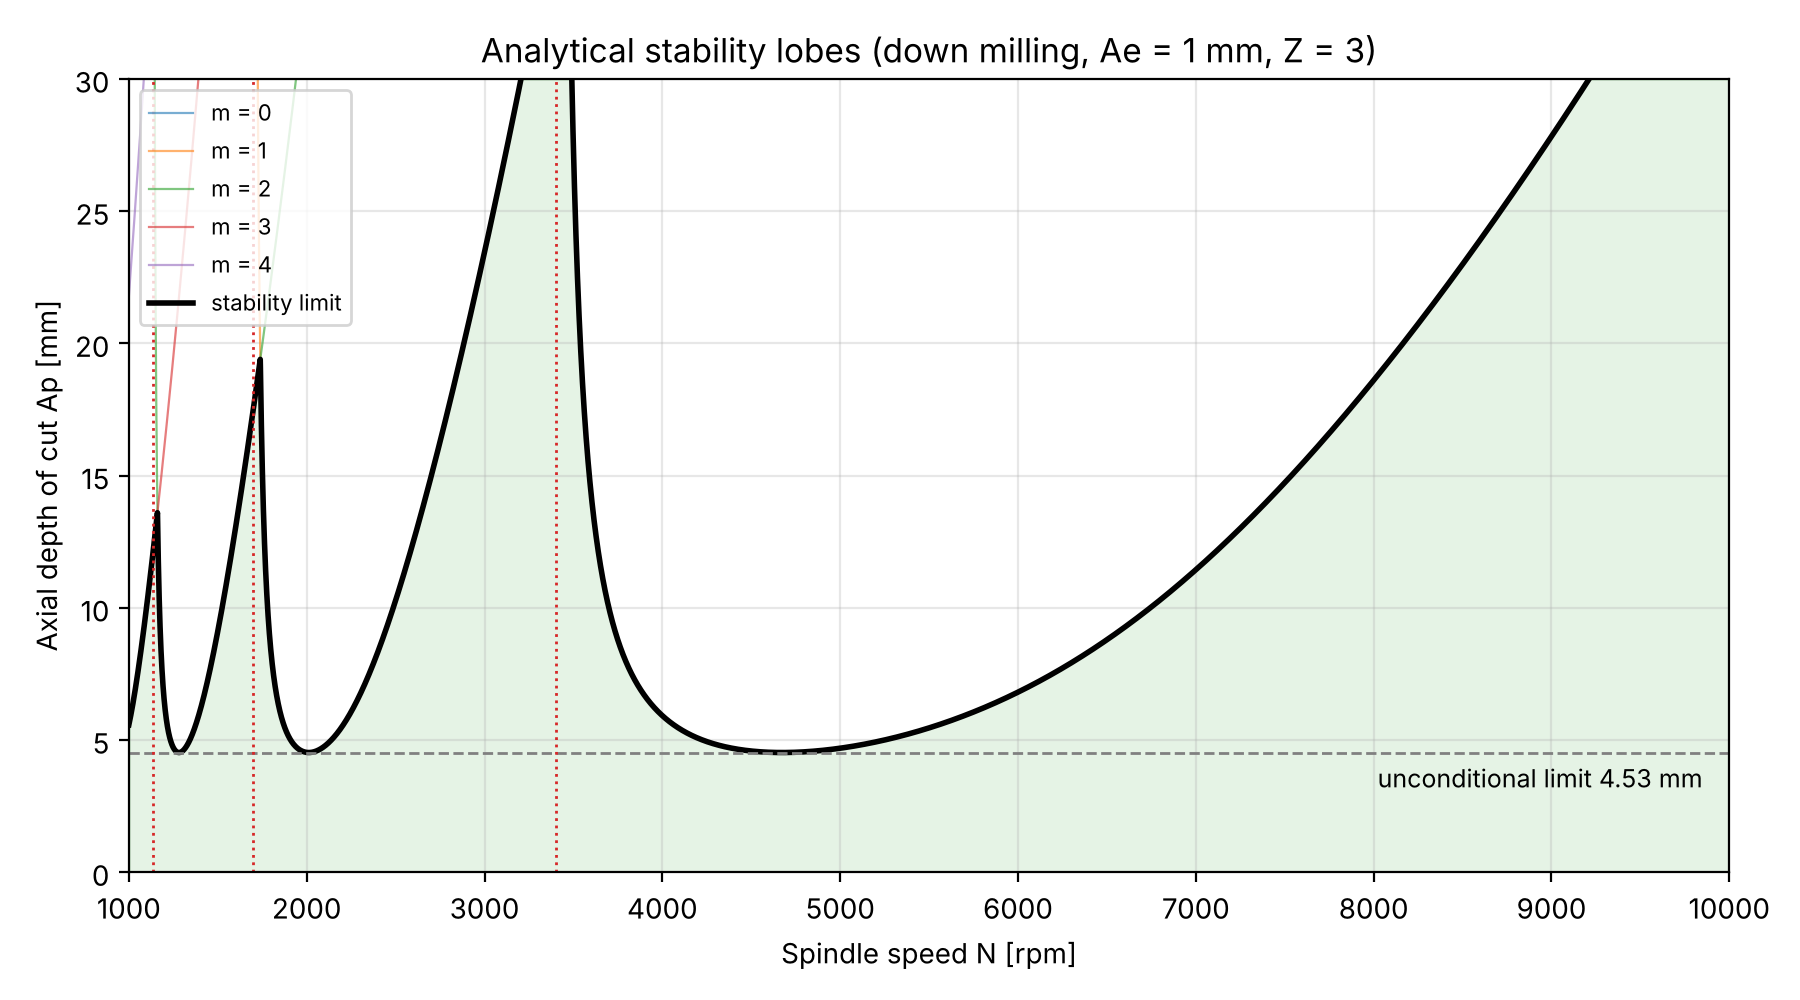
\includegraphics[width=0.9\textwidth]{analytical_lobes.png}
  \caption{Analytical stability lobes (down milling, $A_e=\SI{1}{mm}$). Red dotted lines:
  preferred speeds of question 3.2. Green: stable area.}
  \label{fig:an}
\end{figure}

\begin{itemize}
  \item \textbf{Unconditional limit of stability: $A_{p,lim}=\SI{4.53}{mm}$}, reached for
        a chatter frequency $f_c\approx\SI{176.7}{Hz}$. Below this depth the cut is stable
        at any spindle speed.
  \item \textbf{Optimal spindle speed ranges}: the speeds around the peaks of the lobes,
        where the limit is much higher than the unconditional limit. The peaks are at
        \SI{3469}{rpm} ($m=0$, more than \SI{30}{mm}), \SI{1739}{rpm} ($m=1$, \SI{19.4}{mm})
        and \SI{1161}{rpm} ($m=2$, \SI{13.6}{mm}). They are about \SI{2}{\percent} above the
        preferred speeds of question 3.2 because of the damping. The best range is the one
        around the main lobe ($m=0$), near \SI{3400}{rpm}; above about \SI{6500}{rpm} the
        limit also increases again.
\end{itemize}

\section{Numerical stability lobes}

\subsection{Numerical lobes without helix angle (question 4.1)}
The script \texttt{numerical\_lobes.py} (semi-discretization, Insperger \& St\'ep\'an) was
run with the tutorial data, down milling (\texttt{fist} $=\arccos(2A_e/D-1)$,
\texttt{fiex} $=\pi$), $\eta=0$, \numrange{1000}{10000}~rpm and \numrange{0}{30}~mm.
The modelling parameters entered are: $Z=3$, $D=\SI{20}{mm}$, $K_t=\SI{550}{MPa}$,
$k_r=0.273$, $f_1=\SI{170.0}{Hz}$, $\xi=0.04$, $k=\SI{3.00e6}{N/m}$ and $A_e/D=0.05$.
Before running it, three corrections were made:
\begin{itemize}
  \item \texttt{MC = inv(C)@C} replaced by \texttt{MC = inv(M)@C} (typing mistake, the
        damping term $c/m$ was lost);
  \item the $1\times1$ arrays are used as scalars in \texttt{A[1,0]} and \texttt{B[1,0]}
        (error with numpy 2.x);
  \item the tooth angle is taken modulo $2\pi$ before testing if the tooth is cutting, as
        in the definition of $g_j(t,z)$ (with the helix, the angle can become negative).
\end{itemize}

\begin{figure}[H]
  \centering
  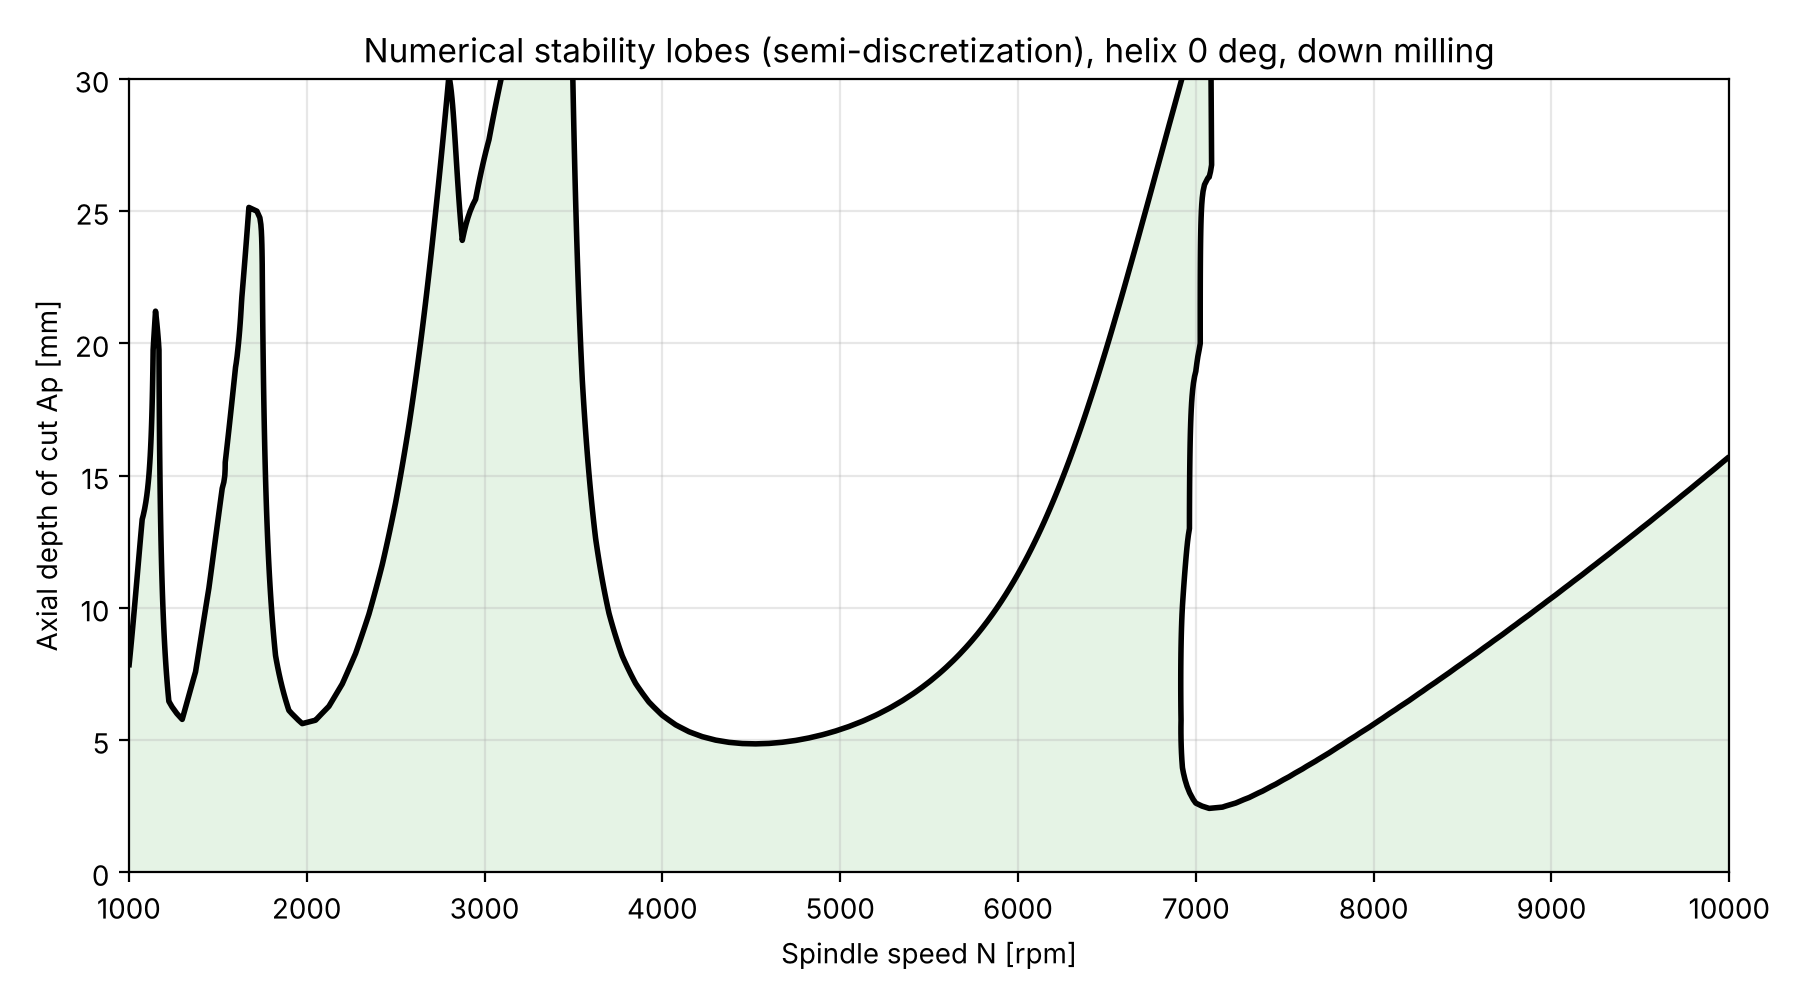
\includegraphics[width=0.85\textwidth]{numerical_helix0_down.png}
  \caption{Numerical stability lobes without helix angle (black line: eigenvalue norm equal to 1).}
  \label{fig:num0}
\end{figure}

\subsection{Comparison with the analytical lobes (question 4.2)}

\begin{figure}[H]
  \centering
  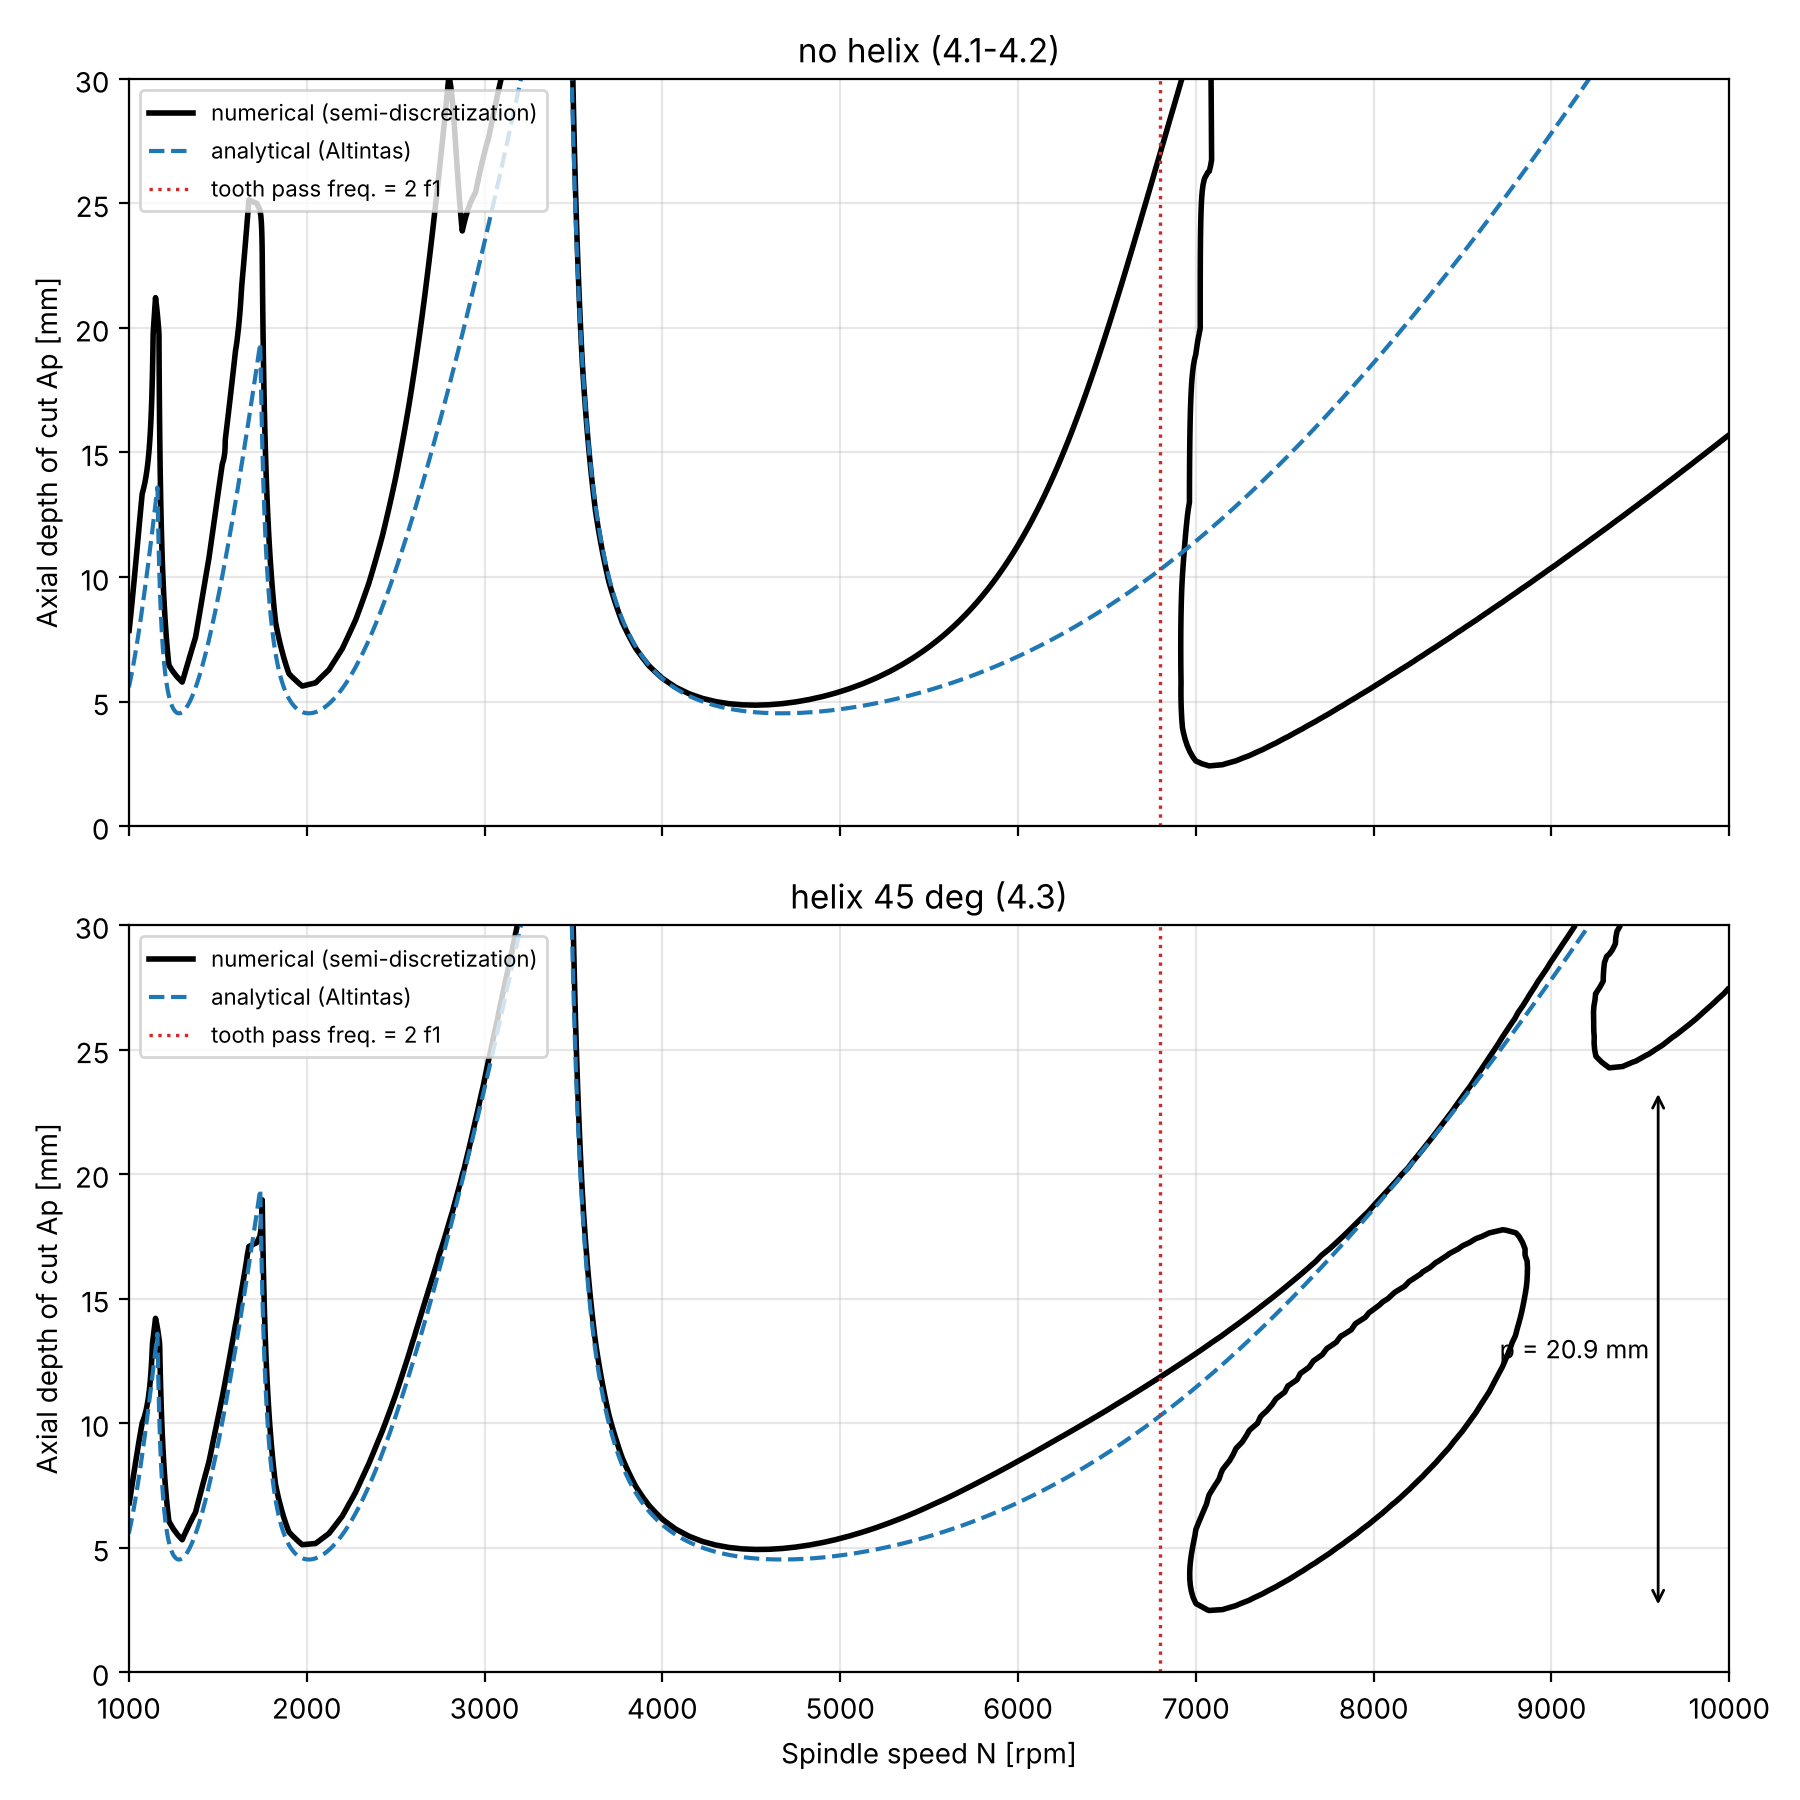
\includegraphics[width=0.85\textwidth]{analytical_vs_numerical.png}
  \caption{Analytical (dashed) and numerical (black) stability lobes, without helix angle
  (top) and with $\eta=\SI{45}{\degree}$ (bottom). Red dotted line: tooth pass frequency equal
  to $2f_1$.}
  \label{fig:comp}
\end{figure}

\begin{itemize}
  \item \textbf{Hopf lobes}: the two models give the same lobes. The numerical minimum is
        \SI{4.85}{mm} (at \SI{4525}{rpm}) against \SI{4.53}{mm} for the analytical model,
        which is slightly conservative; at low speed the numerical peaks are higher.
  \item \textbf{Flip lobe}: the numerical model shows a new unstable zone starting near
        \SI{6900}{rpm}, with a minimum of \textbf{\SI{2.4}{mm} at \SI{7075}{rpm}}, i.e.\ below
        the analytical unconditional limit. The analytical model predicts a stable cut there
        up to about \SI{10}{mm}.
  \item \textbf{Ratio 2} between tooth pass frequency and natural frequency:
        \begin{equation}
        \frac{ZN}{60}=2f_1\quad\Rightarrow\quad N=\frac{2\cdot 170.0\cdot 60}{3}=\SI{6800}{rpm}
        \end{equation}
        This is where the flip lobe begins: it is a period doubling instability.
  \item \textbf{Impact of interrupted milling}: with $A_e/D=0.05$ each tooth cuts only
        \SI{25.8}{\degree} per revolution, i.e.\ $3\times25.8/360\approx\SI{21}{\percent}$ of
        the time, and never two teeth at the same time. The cutting force is a series of
        pulses, very far from the constant average force of the analytical model. The
        analytical approach cannot predict this instability.
\end{itemize}

\subsection{Numerical lobes with helix angle (question 4.3)}
With $\eta=\SI{45}{\degree}$ (Figure~\ref{fig:comp}, bottom):
\begin{itemize}
  \item the Hopf lobes do not change much (minimum \SI{4.93}{mm}) and they are closer to the
        analytical lobes, because the helix spreads the engagement along the tool axis and
        the force becomes more regular;
  \item the flip lobe becomes a \textbf{closed island}, between about \SI{2.5}{mm} and
        \SI{18}{mm} (\numrange{6950}{8850}~rpm), and a second island starts at about
        \SI{24.5}{mm}.
\end{itemize}
The axial pitch of the tool is
\begin{equation}
p=\frac{\pi D}{Z\tan\eta}=\frac{\pi\cdot 20}{3\cdot\tan\SI{45}{\degree}}=\SI{20.9}{mm}
\end{equation}
When $A_p$ is a multiple of $p$, the length of cutting edge in the material is constant
during the rotation, so the directional coefficient $H(t,a_p)$ is constant and there is no
period doubling. Between these depths $H(t,a_p)$ varies again and the flip instability comes
back: this explains the islands, repeated with a period close to $p$ in depth.

\subsection{Conclusion (question 4.4)}
\begin{itemize}
  \item The numerical approach takes into account what the analytical one neglects:
        interrupted cutting (flip lobes) and helix angle (islands). It could also include
        runout or a variable pitch.
  \item For this finishing operation (low $A_e/D$, few teeth) the analytical model is good
        for the Hopf lobes but it is not safe around a tooth pass frequency equal to
        $2f_1$ (\numrange{6800}{8800}~rpm).
  \item In production, the analytical approach is fast and enough for roughing with
        multi-teeth tools and for a first choice of the spindle speed. For finishing with low
        radial immersion, the numerical approach should be used. In both cases the result depends on the identification of the
        dynamic parameters ($f_1$, $k$, $\xi$) and of the cutting coefficients.
\end{itemize}

% ===========================================================================
\part*{Project -- Slot milling}
% ===========================================================================
\section{Data and model}
Slot milling of a 6061-T6 workpiece with a solid carbide end mill: $D=\SI{12}{mm}$, $Z=3$,
$\eta=\SI{45}{\degree}$, cutting length $L_c=\SI{30}{mm}$, overall length $L=\SI{76}{mm}$,
damping $\xi=\SI{1}{\percent}$, maximum spindle speed \SI{6000}{rpm}.

\begin{itemize}
  \item Cutting coefficients: same material as the tutorial, $K_t=\SI{550}{MPa}$,
        $K_r=\SI{150}{MPa}$.
  \item Carbide: $E=\SI{600}{GPa}$, $\rho=\SI{14500}{kg/m^3}$.
  \item The tool is the flexible element. It is modelled as a cantilever cylinder of
        diameter $D$ and free length $l$; tool holder and spindle are rigid. The free length
        cannot be smaller than the cutting length: $l\geq L_c=\SI{30}{mm}$.
  \item Slot milling: full immersion, $\varphi_{st}=0$, $\varphi_{ex}=\pi$, so
        $\alpha_x=\frac12[-\cos2\theta-2k_r\theta-k_r\sin2\theta]_0^\pi=-0.857$
        (up and down milling are both present).
  \item The analytical lobes of the tutorial are used.
  \item Cutting conditions to check: a target axial depth of cut $A_p=L_c/2=\SI{15}{mm}$
        (no value is imposed in the subject); spindle speed $N\leq\SI{6000}{rpm}$, i.e.\
        cutting speed $V_c=\pi D N/1000\leq\SI{226}{m/min}$. Speeds below \SI{1000}{rpm}
        ($V_c<\SI{38}{m/min}$) are not considered.
\end{itemize}

\section{Dynamic parameters}
For a free length $l$ (slide ``Dynamic reminder''):
\begin{equation}
I=\frac{\pi D^4}{64},\qquad k=\frac{3EI}{l^3},\qquad m=\rho\,\frac{\pi D^2}{4}\,l,\qquad
\omega_n=\sqrt{\frac km},\qquad c=2\xi\sqrt{km}
\end{equation}
For example, for $l=\SI{30}{mm}$: $I=\SI{1018}{mm^4}$, $k=\SI{6.79e7}{N/m}$,
$m=\SI{49.2}{g}$, $\omega_n=\SI{37140}{rad/s}$ ($f_1=\SI{5911}{Hz}$), $c=\SI{36.5}{Ns/m}$.

A shorter free length gives a stiffer tool, because $k$ depends on $1/l^3$.

\section{Iterations on the free tool length}
The iteration starts with a long overhang, $l=\SI{46}{mm}$ (\SI{30}{mm} of shank clamped),
and the free length is reduced by \SI{4}{mm} at each step until the minimum value
$l=L_c=\SI{30}{mm}$. The natural frequency of the tool is several kHz, so below
\SI{6000}{rpm} there are only lobes of high order ($m\geq 7$). The Excel file computes only
the orders 0 to 4, which here are above \SI{20000}{rpm}; the same formulas were therefore
computed in Python for all the orders below \SI{6000}{rpm}.

\begin{table}[H]
\centering
\caption{Dynamic parameters and check of the cutting conditions for each free length.
$A_{p,lim}$: unconditional limit; $A_{p,max}$: highest stability limit in
\numrange{1000}{6000}~rpm. Check: at $A_p=\SI{15}{mm}$ there is at least one stable and one
unstable spindle speed.}
\begin{tabular}{ccccccc}
\toprule
$l$ [mm] & $k$ [N/mm] & $m$ [g] & $f_1$ [Hz] & $A_{p,lim}$ [mm] & $A_{p,max}$ [mm] & Check \\
\midrule
\rowsinput{../project/results/iterations_rows.tex}
\bottomrule
\end{tabular}
\end{table}

\begin{figure}[H]
  \centering
  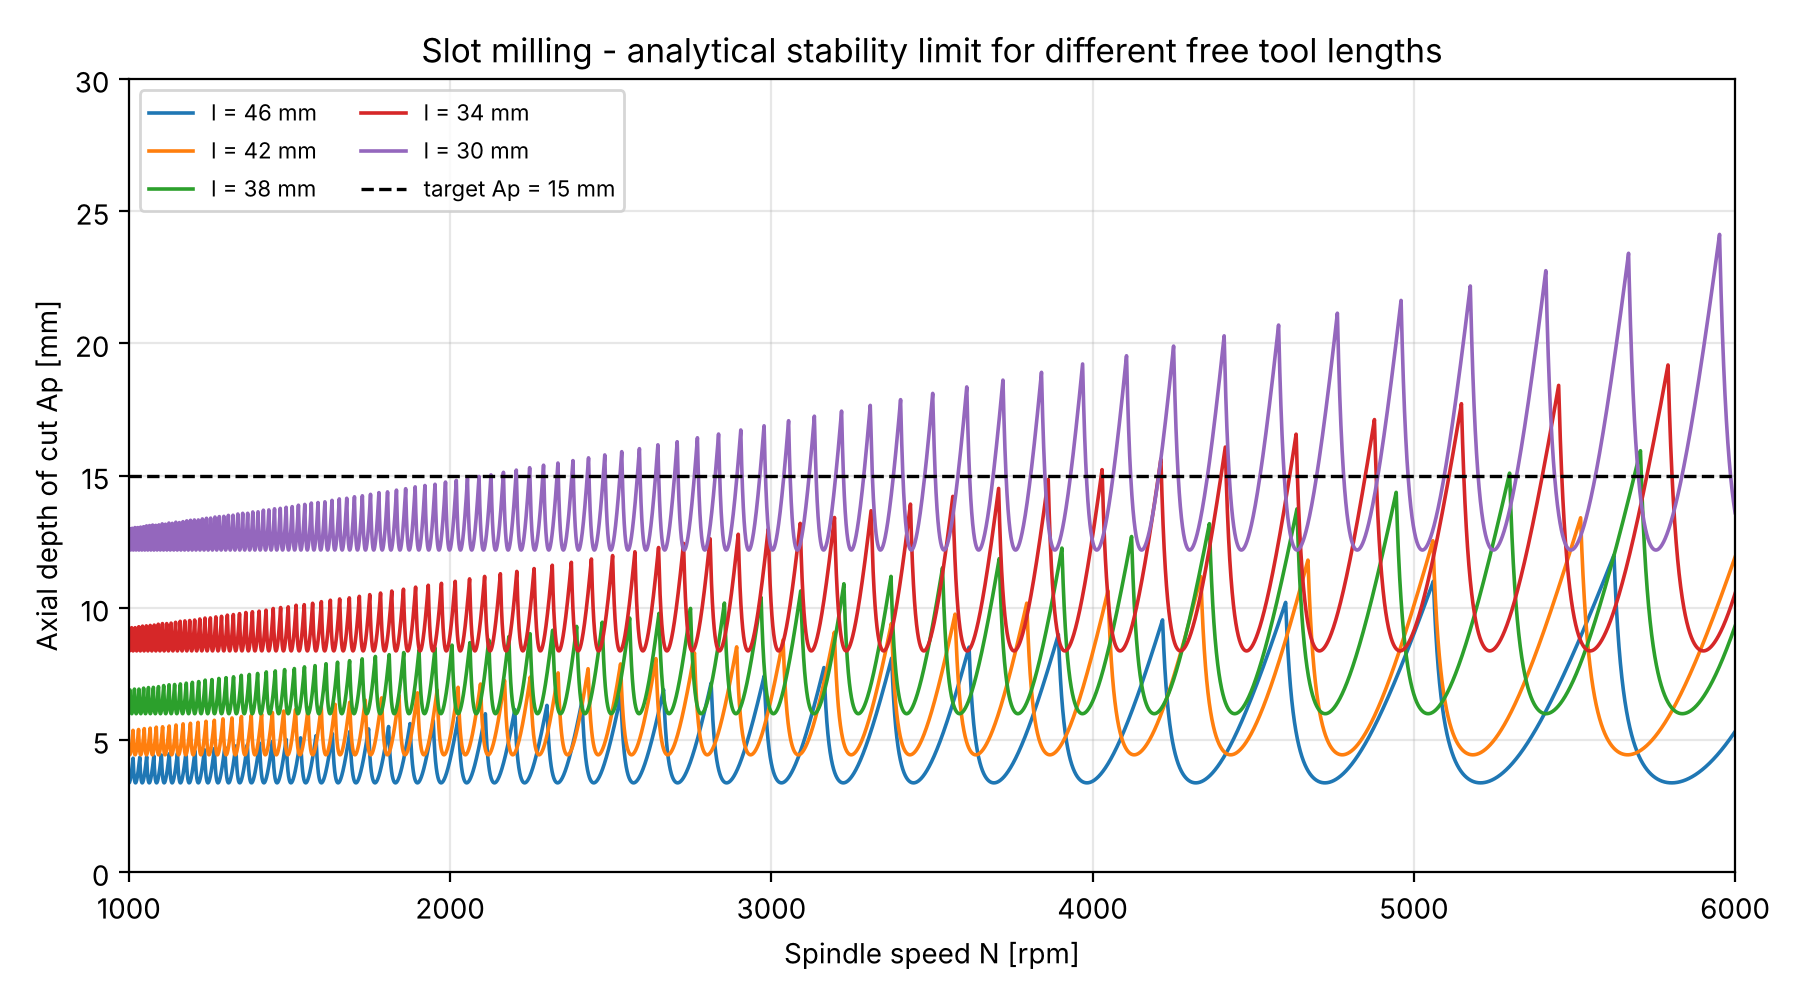
\includegraphics[width=0.9\textwidth]{lobes_free_length.png}
  \caption{Analytical stability limit of the slot milling operation for the different free
  tool lengths.}
  \label{fig:iter}
\end{figure}

\begin{itemize}
  \item $l=46$ and \SI{42}{mm}: the stability limit stays below \SI{15}{mm} in the whole
        speed range, so there is no stable spindle speed. The free length is reduced.
  \item $l=38$ and \SI{34}{mm}: some stable speeds appear and the check is already
        satisfied. As the aim is to increase the stiffness, the free length is still reduced,
        down to its minimum value.
  \item $l=L_c=\SI{30}{mm}$: the stiffness is the highest possible ($k=\SI{67858}{N/mm}$).
        The limit reaches \SI{24.1}{mm} in the speed range, so stable speeds exist; the
        unconditional limit (\SI{12.2}{mm}) is lower than \SI{15}{mm}, so unstable speeds
        also exist. This free length is kept.
\end{itemize}

\section{Selected cutting conditions}

\begin{figure}[H]
  \centering
  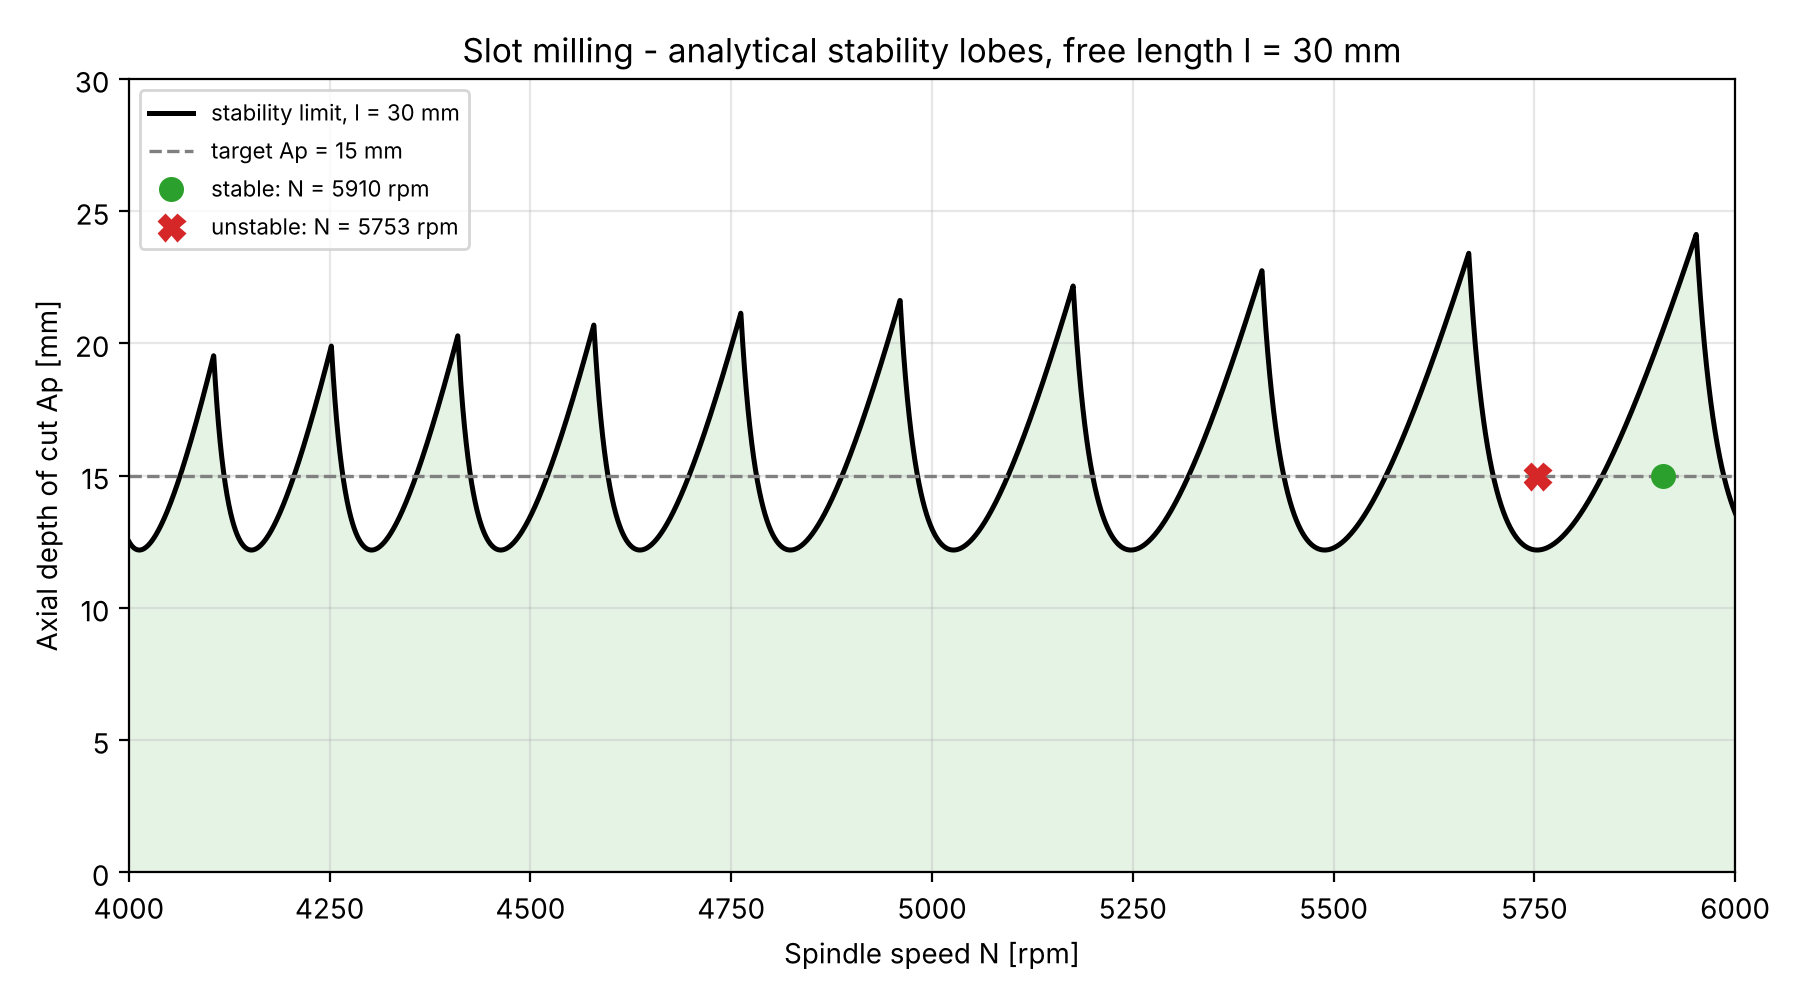
\includegraphics[width=0.9\textwidth]{lobes_final.png}
  \caption{Stability lobes for $l=\SI{30}{mm}$ between 4000 and \SI{6000}{rpm}, with the
  selected stable and unstable spindle speeds at $A_p=\SI{15}{mm}$.}
  \label{fig:final}
\end{figure}

The stable speed is chosen in the stable range closest to the maximum spindle speed, to
have the highest cutting speed. The unstable speed is taken at the bottom of the lobe just
below.

\begin{table}[H]
\centering
\caption{Selected spindle speeds ($l=\SI{30}{mm}$, $A_p=\SI{15}{mm}$, slot milling).}
\begin{tabular}{lcccc}
\toprule
 & $N$ [rpm] & $V_c$ [m/min] & Stability limit [mm] & Result \\
\midrule
Stable & 5910 & 223 & 20.5 & stable \\
Unstable & 5753 & 217 & 12.2 & chatter \\
\bottomrule
\end{tabular}
\end{table}

Both speeds respect $N\leq\SI{6000}{rpm}$ and $V_c\leq\SI{226}{m/min}$. At \SI{5910}{rpm}
the stability limit (\SI{20.5}{mm}) is higher than \SI{15}{mm}, so the cut is stable; at
\SI{5753}{rpm} it is lower (\SI{12.2}{mm}), so the same depth of cut gives chatter.

\section{Conclusion}
For the slot milling operation, the tool is the flexible element. Its stiffness increases
when the free length decreases, so the free length was reduced to its minimum value
$l=L_c=\SI{30}{mm}$. With this length, a slot of \SI{15}{mm} depth can be machined without
chatter at \SI{5910}{rpm} ($V_c=\SI{223}{m/min}$), while \SI{5753}{rpm} is unstable. A depth
of cut below \SI{12.2}{mm} would be stable at any speed.

\end{document}
